\documentclass[11pt]{article}
\RequirePackage{fullpage}
\RequirePackage[font=small,labelfont=bf]{caption}
\RequirePackage{amsmath,amssymb,amsthm}
\RequirePackage{mathtools}
\RequirePackage{graphicx}
\RequirePackage[normalem]{ulem}
\RequirePackage[hidelinks]{hyperref}
\RequirePackage{subcaption}
\RequirePackage{authblk}
\RequirePackage{bm}
\RequirePackage{bbm}
\RequirePackage{tikz}

% line numbers:
\RequirePackage{lineno}
%\modulolinenumbers[5]
\definecolor{linenogray}{gray}{0.75}
\renewcommand\linenumberfont{\normalfont\tiny\sffamily\color{linenogray}}

% spacing
\RequirePackage{setspace}
%\doublespacing
 
% \RequirePackage[osf]{mathpazo}
\RequirePackage[bibstyle=authoryear,citestyle=authoryear-comp,
                date=year,
                maxbibnames=9,maxnames=5,maxcitenames=2,
                backend=biber,uniquelist=false,uniquename=false,
                % style=apa,
                sorting=nyt,
                hyperref=true]{biblatex}
\RequirePackage[colorinlistoftodos]{todonotes}  %disable
\RequirePackage{color}
\RequirePackage{nicefrac}

\newcommand{\gc}[1]{{\it \color{red} #1 } }
\newcommand{\vb}[1]{{\it \color{blue} #1}}
\newcommand{\vbout}[1]{{\it \color{blue} \sout{#1}}}

% a /nonumber you can turn on/off
\newcommand{\nnn}{\nonumber}
%\newcommand{\nnn}{}


\newcommand{\graham}[1]{\todo[size=\scriptsize, color=red!50]{#1}}
\newcommand{\vince}[1]{\todo[size=\scriptsize, color=blue!50]{#1}}

\renewcommand{\P}{\mathbb{P}}
\newcommand{\E}{\mathbb{E}}
\newcommand{\V}{\text{V}}
\newcommand{\cf}{\emph{cf.} }
\DeclareMathOperator{\var}{Var}
\DeclareMathOperator{\cov}{Cov}
\DeclareMathOperator{\T}{{\mathrm{T}}}
\newcommand{\vect}[1]{\mathbf{#1}}
\newcommand{\nssh}{SSH_n}

\newcommand{\chapquote}[2]{\begin{quotation} \textit{#1} \end{quotation} \begin{flushright} - #2\end{flushright} }

\addbibresource{biblio.bib}


% TODO
% - generate figures and write about them

\title{}

\author{}

% \author[$\ast$,$\dag$,$1$]{Vince Buffalo}
% \author[$\dag$]{Graham Coop}
% \affil[$\ast$]{\footnotesize Population Biology Graduate Group}
% \affil[$\dag$]{\footnotesize Center for Population Biology, Department of Evolution and Ecology, University of California, Davis, CA 95616}
% \affil[$1$]{\footnotesize Email for correspondence: \href{mailto:vsbuffalo@ucdavis.edu}{vsbuffalo@ucdavis.edu}}

\begin{document}
\maketitle

\section{Introduction}

\section{Results}


We measure two types of covariances between allele frequency caused by
selection: temporal autocovariances, and across-replicate covariances. First,
positive temporal autocovariance in a neutral allele frequency's trajectory
occurs when the allele becomes associated with a high or low fitness
chromosomal background, and this association persists through the generations
due to linkage disequilibrium. As long as the direction of selection remains
constant, the fitness background is predictive of the direction in the neutral
allele's frequency changes, creating positive covariance. Even though these
magnitude of frequency changes at each site may be subtle, as they would be
under polygenic selection, cumulatively these perturb neighboring sites in a
predictable manner and build up temporal autocovariance which acts as a
genome-wide signal of linked selection. Second, if evolution occurs in
replicate populations undergoing convergent selection pressure, neutral sites
linked to fitness backgrounds shared across replicates are expected to change
in the same direction. This creates across-replicate covariance, which is a
measure of the extent to which convergent selection pressures across replicate
populations cause similar allele frequency changes. Finally, it is important to
note that under the null model where the fitness differences between
individuals are entirely random and non-heritable (e.g. when selection is not
acting), both forms of covariances are expected to be zero. 

Explain G.

We first analyzed \textcite{Barghi2019-qy}, an evolve-and-resequence study with
ten replicate populations exposed to a high temperature environment and evolved
for 60 generations, and sequenced every ten generations. Using the seven
timepoints and ten replicate populations, we estimated a bias-corrected $60
\times 60$ temporal-replicate variance-covariance matrix (see XXX for details).
Since each replicate population was sequenced every ten generations, the
timepoints $t_0 = 0$ generations, $t_1 = 10$ generations, $t_2 = 20$
generations, etc., lead to observed allele frequency changes across ten
generation chunks, $\Delta p_{t_0}, \Delta p_{t_1}, \ldots, \Delta p_{t_6}$.
Consequently, the ten temporal covariance matrices for each of the ten
replicate populations have off-diagonal elements of the form $\cov(\Delta
p_{t_0}, \Delta p_{t_1}) = \cov(p_{t_1} - p_{t_0}, p_{t_2} - p_{t_1}) =
\sum_{i=0}^{10} \sum_{j=10}^{20} \cov(\Delta p_i, \Delta p_j)$. Each diagonal
element has the form $\var(\Delta p_{t_0}) = \sum_{i=0}^{t_0} \var(\Delta
p_{i}) + \sum_{i \ne j}^{t_0} \cov(\Delta p_{i}, \Delta p_{j})$, and is thus a
combination of the effects of drift and selection, as both the variance in
allele frequency changes and cumulative temporal autocovariances terms increase
the variance in allele frequency. With sampling each generation, one could more
accurately partition the total variance in allele frequency change
\parencite{Buffalo2019-io}; while we cannot directly estimate the contribution
of linked selection to the variance in allele frequency change here, the
presence of a positive observed covariance between allele frequency change can
only be caused linked selection. 

Averaging across replicate populations, we find positive temporal covariances
that are statistically significant (p < XXX) consistent with linked selection
acting to affect allele frequency changes over very short time periods. We
visualize these covariances in Figure \label{figure-1} (A), which depicts the
temporal covariances through time, for each of the five rows covariance matrix.
Each row represents the temporal covariance $\cov(\Delta p_s, \Delta p_t)$,
between some initial reference generation $s$ (the row of the matrix), and some
later timepoint $t$ (the column of the matrix). For each row, the covariances
at first are positive, and then decay towards zero as expected when directional
selection affects linked variants' frequency trajectories until ultimately
linkage disequilibrium and additive genetic variance for decay
\parencite{Buffalo2019-io}.


we can calculate the temporal
covariances between an initial starting reference generation ($s = \{0, 10, 20,
\ldots, 50\})$.

\begin{figure}[!ht]
  \centering
  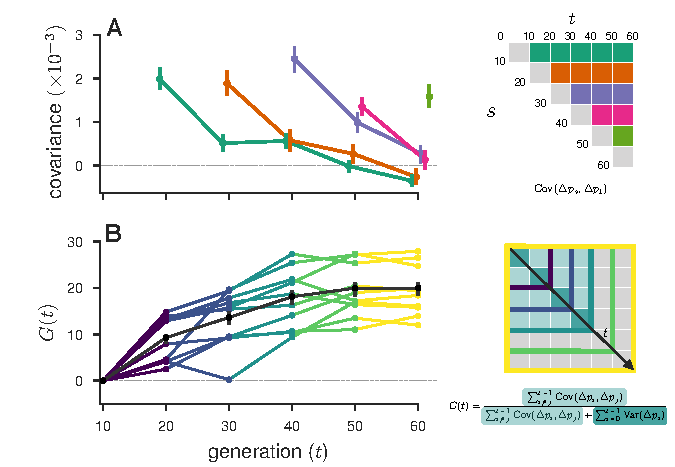
\includegraphics[width=\textwidth]{figures/figure-1.pdf}
  \caption{$B=5000$ bootstraps, with 100}
  \label{fig:figure-1}
\end{figure}

\begin{figure}[!ht]
  \centering
  \includegraphics[width=\textwidth]{}
  \caption{}
  \label{}
\end{figure}


\begin{figure}[!ht]
  \centering
  \includegraphics[width=\textwidth]{}
  \caption{}
  \label{}
\end{figure}


\begin{figure}[!ht]
  \centering
  \includegraphics[width=\textwidth]{}
  \caption{}
  \label{}
\end{figure}


\section{Appendix}

\section{Sampling Bias Corrections}

Following \textcite{Waples1989-sj}, we have that that the variance in the
initial generation, which is entirely due to the binomial sampling process, is
$\var(p_0) = \nicefrac{p_0(1-p_0)}{d_0}$ where $d_0$ is the number of binomial
draws (e.g. read depth). At a later timepoint, the variance in allele frequency
is a result of both the binomial sampling process at time $t$ and the
evolutionary process.

Using the law of total variation, 

\begin{align}
  \var(\widetilde{p_t}) &= \E(\var(\widetilde{p_t} | p_t)) + \var(\E(\widetilde{p_t}|p_t)) \\
                        &= \underbrace{\frac{p_t(1-p_t)}{d_t}}_\text{generation $t$ sampling noise} + \underbrace{\var(p_t)}_\text{variance due to evolutionary process}
  %\frac{\var(\widetilde{p_t})}{p_0(1-p_0)} &= \frac{p_t(1-p_t)}{p_0(1-p_0) d_t} + 1 - \left( 1-\frac{1}{2N}\right)^t.
  %\frac{\var(\widetilde{p_t})}{p_0(1-p_0)} &= \frac{p_t(1-p_t)}{p_0(1-p_0) d_t} + \frac{t}{2N} + O\left((2 N)^{-2}\right).
\end{align}

Under a drift-only process, $\var(p_t) = p_0(1-p_0)\left[1- \left(1 -
\frac{1}{2N}\right)^t\right]$. However, with heritable variation in fitness, we
need to consider the covariance in allele frequency changes across generations
\parencite{Buffalo2019-io}. We can write

\begin{align}
  V(p_t) &= V\left(p_0 + (p_1 - p_0) + (p_2 - p_1) + \ldots + (p_t - p_{t-1}) \right) \\
         &= V\left(p_0 + \Delta p_0 + \Delta p_1 + \ldots + \Delta p_{t-1} \right) \\
         &= V(p_0) + \sum_{i=0}^{t-1} \cov(p_0, \Delta p_i) + \sum_{i=0}^{t-1} \var(\Delta p_i) + \sum_{0 \le i < j}^{t-1} \cov(\Delta p_i, \Delta p_j).
\end{align}
%

Each allele frequency change is equally like to be positive as it is to be
negative; thus by symmetry this second term is zero. Additionally $V(p_0) = 0$,
as we treat $p_0$ as a fixed initial frequency. We can write, 

\begin{align}
  V(p_t) &= \sum_{i=0}^{t-1} \var(\Delta p_i) + \sum_{0 \le i < j}^{t-1} \cov(\Delta p_i, \Delta p_j).
\end{align}

The second term, the cumulative impact of variance in allele frequency change
can be partitioned into heritable fitness and drift components
\parencite{Santiago1995-hx,Buffalo2019-io}

\begin{align}
  V(p_t) &= \sum_{i=0}^{t-1} \var(\Delta_{_D} p_i) + \sum_{i=0}^{t-1} \var(\Delta_{_H} p_i) + \sum_{0 \le i < j}^{t-1} \cov(\Delta p_i, \Delta p_j).
\end{align}

where $\Delta_{_H} p_t$ and $\Delta_{_D} p_t$ indicate the allele frequency
change due to heritable fitness variation and drift respectively. Then, sum of
drift variances in allele frequency change is

\begin{align}
  \sum_{i=0}^{t-1} \var(\Delta_{_D} p_i) = \sum_{i=0}^{t-1} \frac{p_i(1-p_i)}{2N}
\end{align}

replacing the heterozygosity in generation $i$ with its expectation, we have

\begin{align}
  \sum_{i=0}^{t-1} \var(\Delta_{_D} p_i) &= p_0(1-p_0) \sum_{i=0}^{t-1} \frac{1}{2N} \left(1-\frac{1}{2N}\right)^i \\
                                         &= p_0(1-p_0) \left[1 - \left(1-\frac{1}{2N}\right)^t \right]
\end{align}

which is the usual variance in allele frequency change due to drift.  Then, the
total allele frequency change from generations $0$ to $t$ is
$\var(\widetilde{p}_t - \widetilde{p}_0) = \var(\widetilde{p}_t) +
\var(\widetilde{p}_0) - 2 \cov(\widetilde{p}_t, \widetilde{p}_0)$, where the
covariance depends on the nature of the sampling plan (see \cite{Nei1981-oy,
Waples1989-sj}). In the case where there is heritable variation for fitness,
and using the fact that $\cov(\widetilde{p}_t, \widetilde{p}_0) =
\nicefrac{p_0(1-p_0)}{2N}$ for Plan I sampling procedures
\parencite{Waples1989-sj}, we write,

\begin{align}
  \var(\widetilde{p}_t - \widetilde{p}_0) &= \var(\widetilde{p}_t) + \var(\widetilde{p}_0) - 2 C \cov(\widetilde{p}_t, \widetilde{p}_0) \\
                                          &= \frac{p_t(1-p_t)}{d_t}  + \frac{p_0(1-p_0)}{d_0} + p_0(1-p_0) \left[1 - \left(1-\frac{1}{2N}\right)^t \right] + \\ & \;\;\;\;\;\;
                                               \sum_{i=0}^{t-1} \var(\Delta_{_H} p_i)  + \sum_{0 \le i < j}^{t-1} \cov(\Delta p_i, \Delta p_j) - \frac{C p_0(1-p_0)}{2N} \\
  \frac{\var(\widetilde{p}_t - \widetilde{p}_0)}{p_0(1-p_0)} &= 1 + \frac{p_t(1-p_t)}{p_0(1-p_0)d_t}  + \frac{1}{d_0} - \left(1-\frac{1}{2N}\right)^t + \\ & \;\;\;\;\;\;
  \sum_{i=0}^{t-1} \frac{\var(\Delta_{_H} p_i)}{p_0(1-p_0)}  + \sum_{0 \le i < j}^{t-1} \frac{\cov(\Delta p_i, \Delta p_j)}{p_0(1-p_0)} - \frac{C}{N}
\end{align}

where $C = 1$ if Plan I is used, and $C=0$ if Plan II is used (see
\cite{Waples1989-sj}, p. 380 and Figure 1 for a description of these sampling
procedures). We move terms creating a corrected estimator for the population
variance in allele frequency change, and replace all population heterozygosity
terms with the unbiased sample estimators, e.g. $\frac{d_t}{d_t-1}
\widetilde{p}_t (1- \widetilde{p}_t)$,

\begin{align}
  \frac{d_0-1}{d_0} \frac{\var(\widetilde{p}_1 - \widetilde{p}_0)}{\widetilde{p}_0(1-\widetilde{p}_0)} - \frac{(d_0-1)}{d_0 (d_1 - 1)} \frac{\widetilde{p}_1(1-\widetilde{p}_1)}{\widetilde{p}_0(1-\widetilde{p}_0)} - \frac{1}{d_0} + \frac{C}{N}  &= \frac{\var(\Delta_{_H} p_0)}{p_0(1-p_0)} + \frac{1}{2N} 
\end{align}

\subsection{Individual and depth sampling process}

$X_t \sim \text{Binom}(n_t, p_t)$ where $X_t$ is the count of alleles and $n_t$
is the number of diploids sampled at time $t$. Then, these individuals are
sequenced at a depth of $d_t$, and $Y_t \sim \text{Binom}(d_t,
\nicefrac{X_t}{n_t})$ reads have the tracked allele. We let $\widetilde{p_t} =
\nicefrac{Y_t}{d_t}$ be the observed sample allele frequency. Then, the
sampling noise is 

\begin{align}
  \var(\widetilde{p_t}|p_t) &= \E(\var(\widetilde{p_t} | X_t)) + \var(\E(\widetilde{p_t} | X_t)) \\
                            &= p_t(1-p_t) \left(\frac{1}{n_t} + \frac{1}{d_t} - \frac{1}{n_t d_t} \right).
\end{align}

(see also \cite{Jonas2016-ia}).

\begin{align}
  \var(\widetilde{p}_t - \widetilde{p}_0) &= 
  p_t(1-p_t) \left(\frac{1}{n_t} + \frac{1}{d_t} - \frac{1}{n_t d_t} \right)  
  + p_0(1-p_0) \left( \frac{1}{n_0} + \frac{1}{d_0} - \frac{1}{n_0 d_0}\right)  \\ & \;\;\;\;\;\;
  - \frac{C p_0(1-p_0)}{N} + p_0(1-p_0) \left[1 - \left(1-\frac{1}{2N}\right)^t \right]+ \sum_{i=0}^{t-1} \var(\Delta_{_H} p_i)  \\ & \;\;\;\;\;\; + \sum_{0 \le i < j}^{t-1} \cov(\Delta p_i, \Delta p_j) 
\end{align}

Through the law of total expectation, one can find that an unbiased estimator
of the heterozygosity is 

\begin{align}
  \frac{n_t d_t}{(n_t-1) (d_t-1)} \widetilde{p_t}(1-\widetilde{p_t})
\end{align}


\begin{align}
  \var(\widetilde{p}_t - \widetilde{p}_0) &= 
  \frac{n_t d_t \widetilde{p}_t(1-\widetilde{p}_t)}{(n_t-1)(d_t-1)} \left(\frac{1}{n_t} + \frac{1}{d_t} - \frac{1}{n_t d_t} \right) + 
 \frac{n_0 d_0 \widetilde{p}_0(1-\widetilde{p}_0)}{(n_0-1)(d_0-1)} \left( \frac{1}{n_0} + \frac{1}{d_0} - \frac{1}{n_0 d_0}\right) + \\ & \nonumber\;\;\;\;\;\;
 \frac{n_0 d_0 \widetilde{p}_0(1-\widetilde{p}_0)}{(n_0-1)(d_0-1)}   \left[1 - \left(1-\frac{1}{2N}\right)^t \right]  - \frac{C}{N}  \frac{n_0 d_0 \widetilde{p}_0(1-\widetilde{p}_0)}{(n_0-1)(d_0-1)} + \\ \nonumber & \;\;\;\;\;\; \sum_{i=0}^{t-1} \var(\Delta_{_H} p_i)  + \sum_{0 \le i < j}^{t-1} \cov(\Delta p_i, \Delta p_j)  \\
                                                                                                                      &= \widetilde{p}_t(1-\widetilde{p}_t)\frac{d_t + n_t - 1}{(n_t-1)(d_t-1)} + 
 \widetilde{p}_0(1-\widetilde{p}_0)\frac{d_0 + n_0 - 1}{(n_0-1)(d_0-1)} + \\ & \nonumber\;\;\;\;\;\;
 \widetilde{p}_0(1-\widetilde{p}_0) \frac{n_0 d_0}{(n_0-1)(d_0-1)}  \left[1 - \left(1-\frac{1}{2N}\right)^t \right] - \frac{C}{N} \widetilde{p}_0(1-\widetilde{p}_0)\frac{n_0 d_0}{(n_0-1)(d_0-1)} 
 \\ \nonumber & \;\;\;\;\;\; + \sum_{i=0}^{t-1} \var(\Delta_{_H} p_i)  + \sum_{0 \le i < j}^{t-1} \cov(\Delta p_i, \Delta p_j) \
\end{align}


\subsection{Covariance Correction}

We also need to apply a bias correction to the temporal covariances (and
possibly the replicate covariances if the initial sample frequencies are all
shared).

The basic issue is that $\cov(\Delta \widetilde{p}_t, \Delta
\widetilde{p}_{t+1}) = \cov(\widetilde{p}_{t+1} - \widetilde{p}_t,
\widetilde{p}_{t+2} - \widetilde{p}_{t+1})$, and thus shares the sampling noise
of timepoint $t+1$. Thus acts to bias the covariance by subtracting off the
noise variance term of $\var(\widetilde{p}_{t+1})$, so we add that back in.

\subsection{Variance-Covariance Matrix Correction}

With frequency collected at $\tau$ timepoints across $R$ replicate populations
at $L$ loci, we have an $R \times \tau \times L$ array $\mathbf{F}$ of allele
frequencies and $\mathbf{D}$ array of sequencing depths. We calculate the 


change the
dimensionality of

\subsection{Block Bootstrap Procedure}
\label{supp:block-bootstrap}

\end{document}
